\chapter{Diseño del software} \label{chap:SW}
\chapterimage{figuras/ImagenesPortada/PortadaSW.jpg}
\hrule
\vspace{3mm}

Este capítulo cubre el diseño e implementación del software que hace efectivo el estudio matemático y el control descrito anteriormente para el brazo robótico.
\\
El capítulo presenta unos aspectos generales así como una filosofía de diseño a implementar para posteriormente hacer una descripción detallada de los distintos componentes implementados. Finalmente se hace una justificación de los test que se han efectuado sobre los diferentes componentes así como un análisis de la correcta gestión de la complegidad y mantenimiento que se plantea inicialmente.

\section{Filosofía de diseño} \label{sec:SW:filosofia_diseño}

\completarCon{REGLAS DE CODIFICACION, GESTION COMPLEJIDAD Y PATRONES DE DISEÑO}

\section{Aspectos generales del diseño} \label{sec:SW:diseño_general}

El software del proyecto está separado en diferentes componentes que interactuan entre si para realizar las diferentes funcionalidades necesarias. Como se ha explicado en el capítulo \ref{chap:Control} se han implementado diferentes lazos de control a diferentes niveles que serán coordinados a diferentes frecuencias.
\\
Es importante recordar del capítulo \ref{chap:Electronica} la necesidad de interactuar con un protocolo de comunicación a bajo nivel con los Servos. Este protocolo se encuentra explicado en detalle en el anexo \ref{app:registros_g15}. Siguiendo esta misma línea de trabajo se ha implementado a otro nivel superior un protocolo de comunicación que permitirá la comunicación y control del brazo robótico con cualquier dispositivo externo a través de un puerto serie estándar.
\\
La librería suministrada por el fabricante de los servos, vista en \cite{} \completar se ha utilizado a modo de ejemplo para la implementación de la nueva estructura de control de los servos. Esta librería se caracteriza por implementar un objeto a modo de controlador del puerto serie de forma que irán invocado los diferentes métodos incluidos en la librería completando con la información a enviar. Esta filosofía difiere con la filosofía de diseño que se pretende aplicar en este proyecto.
\\
El diseño del \ingles{software} del brazo robótico pasa por separar la información de la comunicación. Se define un objeto servo que contendrá toda la información referente al mismo y será el en cargado de actualizar los comandos a enviar en base a la información contenida que será actualizada ciclicamente.
\\
De esta forma es necesario crear otro objeto encargado de gestionar la comunicación, de todos los servos, a través del puerto serie.
\\
De forma general se puede decir que los objetos de más alto nivel están encargados de efectuar la actualización de los datos de las clases de más bajo nivel para que estas, con la información que poseen de si mismas efectuen los cálculos correspondientes. Se desarrollará en profundidad este aspecto en los apartados a continuación.

\section{Estructura de directorios y ficheros} \label{sec:SW:estructura_dir}

Para el desarrollo y test del software se ha utilizado el editor \glosario{Atom}, presentado anteriormente en el capítulo \ref{chap:Introduccion}, ampliando su funcionalidad con el paquete \glosario{PlatformIO}, que expande las capacidades del editor base convirtiéndolo en un entorno de desarrollo integrado (IDE) que permite trabajar software embebido \completarCon{Añadir alguna definición?}, entre ellas las de la gama \glosario{Arduino}.
\\

La elección de esta herramienta conlleva un formato en el árbol de directorios en los que se separa el código debido a la forma que tiene de compilar y lincar los diferentes ficheros. De esta manera y para mantener el orden los ficheros de código se separan en tres grandes directorios:

\begin{itemize}
    \item lib: directorio donde se introducen, en carpetas, las librerías o componentes que se van a utilizar.
    \item src: directorio donde se introduce el fichero o ficheros de código principales.
    \item test: directorio donde se introducen los ficheros donde se codifican los test. Estos irán introducidos a su vez dentro de directorios con el nombre de cada test.
\end{itemize}

Concretamente, en el caso de este proyecto y anticipando los componentes que lo componeen, el árbol de directorios queda con la  estructura mostrada a continuación. En algunos casos y a modo de ejemplo se ha llegado hasta un nivel de ficheros. Adicionalmente hay otros directorios donde se almacena información y utilides que se explican más adelante.

\lstset{language=C, breaklines=true, basicstyle=\footnotesize}
    %Introducir label y caption
    \begin{lstlisting}[frame=single]

 -- Sw
 |-- lib
 |   |-- chuck_handler
 |   |-- cytron_g15_servo  // A modo de ejemplo
 |   |-- debug
 |   |   | + debug.cpp
 |   |   | + debug.h
 |   |-- joint_handler
 |   |   | + joint_handler.cpp
 |   |   | + joint_handler.h
 |   |-- joint_rha
 |   |-- memory_free
 |   |-- rha_types
 |   |-- robot_rha
 |   |-- servo_rha
 |   |-- utilities
 |   |-- readme.txt
 |-- src
 |   |-- main.cpp
 |   |-- main_utilities.cpp
 |-- test
 |   |-- a_test_rha_types
 |   |   | + test_rha_types.cpp
 |   |-- b_test_pid_regulator
 |   |-- d_test_servo_rha
 |   |-- e_test_joint_rha
 |   |-- f_test_joint_handler_mock
 |-- platformio.ini
 -------  // Hasta aqui la estructura impuesta por la herramienta platformio
 |-- code_analysis
 |-- utilities
 |-- sw_documentation
 |-- makeAnalysis.sh
    \end{lstlisting}

\section{Descripción de componentes} \label{sec:SW:descripcion_componentes}

Como se ha explicado anteriormente el software del brazo robótico se puede separar en diferentes componentes y utilidades que se procede a explicar a continuación.
    \subsection{Utilidades de debug} \label{subsec:SW:debug}
        No se trata de un componente propiamente dicho si no de una serie de \ingles{macros} que permiten, mediante directivas al precompilador activar mensajes de debug para los diferentes componentes de forma independiente. Cabe destacar que estos mensajes de debug se emiten utilizando el puerto serie por defecto a través de los pines 0 y 1 de la placa tal y como se ha descrito en la sección \ref{sec:Electronica:Placa}. Se debe tener en cuenta que el uso de estas funcionalidades incrementa notablemente el uso de memoria RAM y FLASH de la placa.
        \\
        Activar o desactivar dichas funcionalidades supone comentar o descomentar las directivas referentes a cada componente.  Concretamente, a modo de ejemplo, estas tienen el siguiente aspecto:
        \lstset{language=C, breaklines=true, basicstyle=\footnotesize}
        %Introducir label y captio
        \begin{lstlisting}[frame=single]

    // #define DEBUG_SERVO_RHA
    // #define DEBUG_TEST_SERVO_RHA_REAL

        \end{lstlisting}
    \subsection{Tipos de datos propios del proyecto} \label{subsec:SW:rhatypes}
        Para facilitar el traspaso de información como la codificación del software se han implementado diferentes tipos de dato genéricos para ser utilizados en las diferentes capas de software. Concretamente se han implementado los siguientes componentes cuyos diagramas de clases se puden ver en la figura \ref{fig:SW:class_diagram_TRHA}:

        \begin{itemize}
            \item \ingles{SpeedGoal} condensa en un solo objeto toda la información necesaria para codificar un objetivo de velocidad.
            \item \ingles{Point3} permite un uso más cómodo de coordenadas con tres componentes ya sean articulares de posición o cartesianas.
            \item \ingles{Regulator} encapsula el funcionamiento de un \glosario{Regulador-PID} estandar. Guarda los valores de las constantes así como de la integral del error para luego, introduciendo el valor del error, derivada del error e integral del error en un intervalo poder obtener el valor de la consigna a la salida del regulador.
            \item \ingles{Timer} codifica un temporizador (en milisegundos) de forma que se le podrá preguntar al objeto si el tiempo ya ha pasado, bloqueando o no la ejecución del programa hasta el final de dicho intervalo.
            \item \ingles{TimerMicroseconds} hereda las características del objeto \ingles{Timer} implementando la funcionalidad en microsegundos.
        \end{itemize}

        \begin{figure}[H]
            \centering
            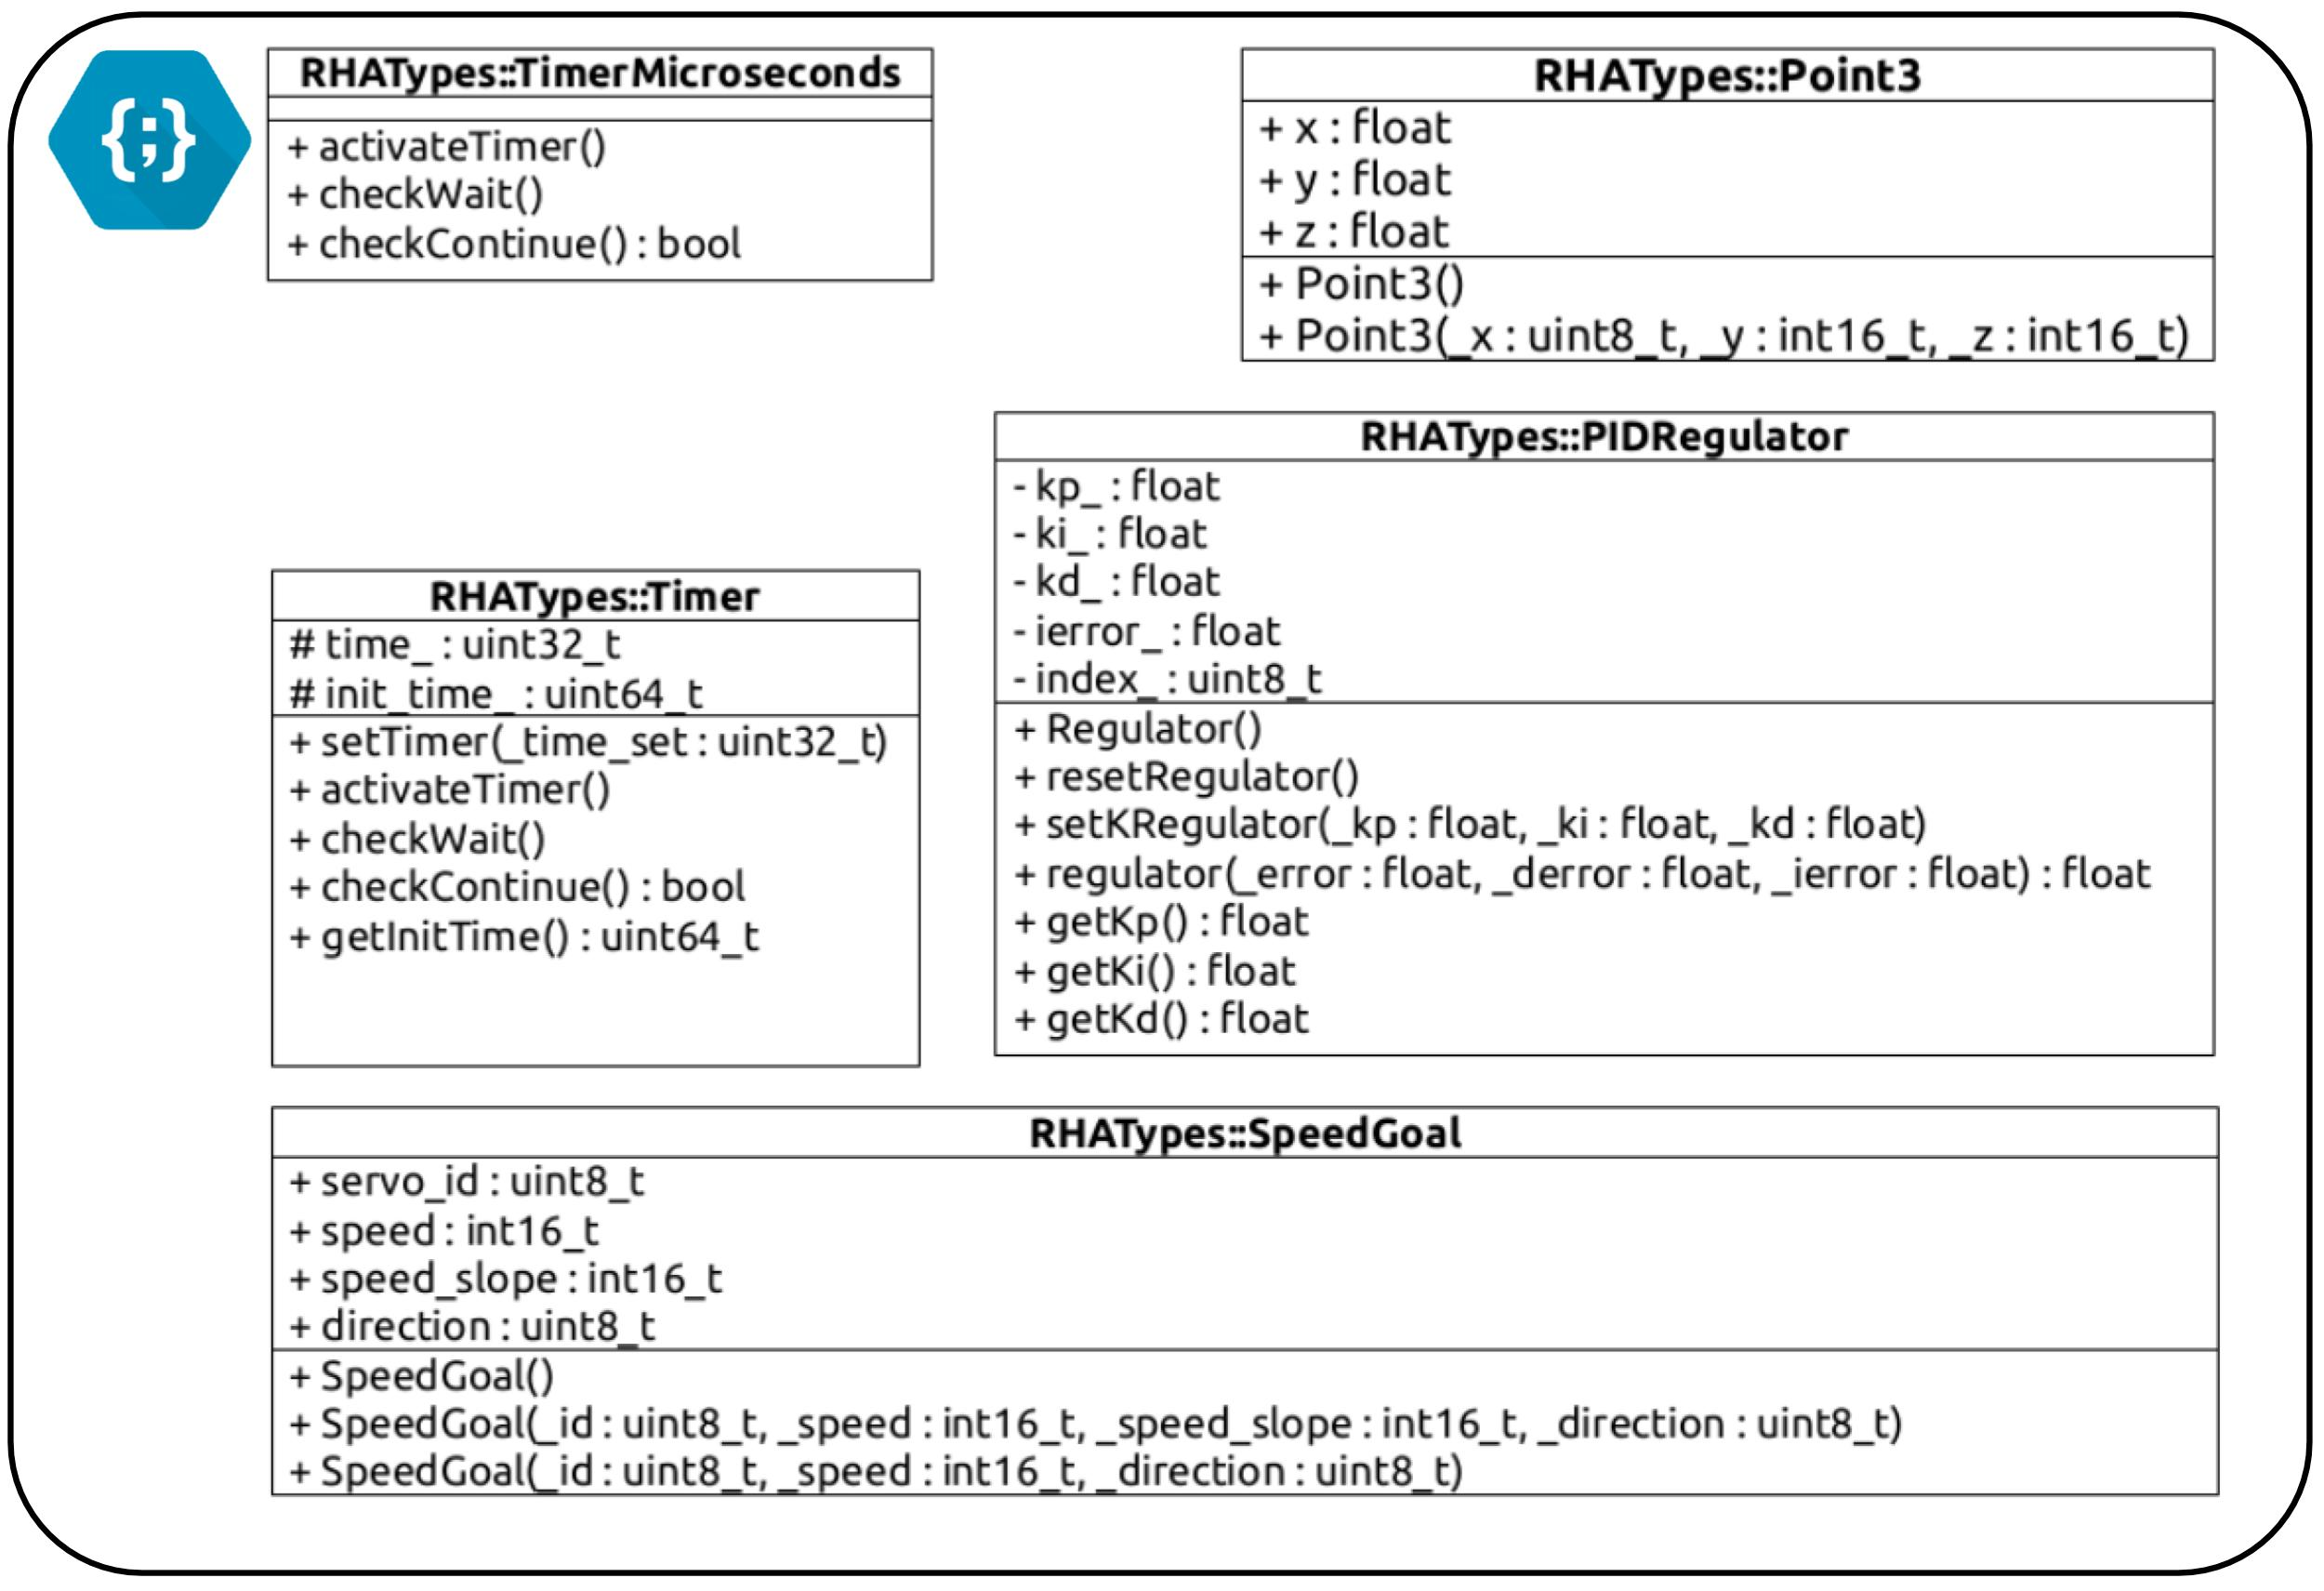
\includegraphics[width=1\textwidth]{figuras/Imagenes_SW/class_diagram_TRHA.jpg}
            \caption{Estructuras de datos auxiliares}
            \label{fig:SW:class_diagram_TRHA}
            \immagesource{Autor}
        \end{figure}

        Se puede consultar información de más bajo nivel referente a estos tipos de datos en el anexo \ref{app:documentacion_software} que agrupa documentacón de todo el software, concretamente en la sección \completar se encuentra la información de los componentes descritos en este apartado.

    \subsection{Gestión de la información del servo} \label{subsec:SW:servorha}
        Como ya se ha anticipado el objeto de tipo ServoRHA (como se ha nombrado internamente) es el encargado de gestionar toda la información referente al servo así como de realizar los cálculos necesarios que involucren dicha información. A petición de objetos de capas superiores encapsula la información que se requiera en un \ingles{buffer} o un vector con los valores correspondientes, siguiendo siempre una estructura concreta para facilitar posterior comunicación con los servos físicos. Como es común en este tipo de objetos posee todo tipo de métodos para acceder a la información almacenada.
        \\
        La información se actualiza, encapsulada en un buffer con un orden concreto, a través de un método concreto que suministra este componente.
        \\
        Desde el punto de vista de control gestiona una parte importante referente al lazo de control de velocidad del servo siendo el encargado en realizar los cálculos necesarios así como de almacenar los valores de consigna a requerir. El objeto \ingles{ServoRHA} instancia un objeto del tipo Regulador visto en la sección \ref{subsec:SW:rhatypes} inicializado con las constantes de control concretas al servo. En el diagrama de la figura \ref{fig:SW:class_diagram_SRHA} se pueden ver los diferentes métodos que hacen efectiva la implementación del lazo de control de velocidad de los servos.

        \begin{figure}[H]
            \centering
            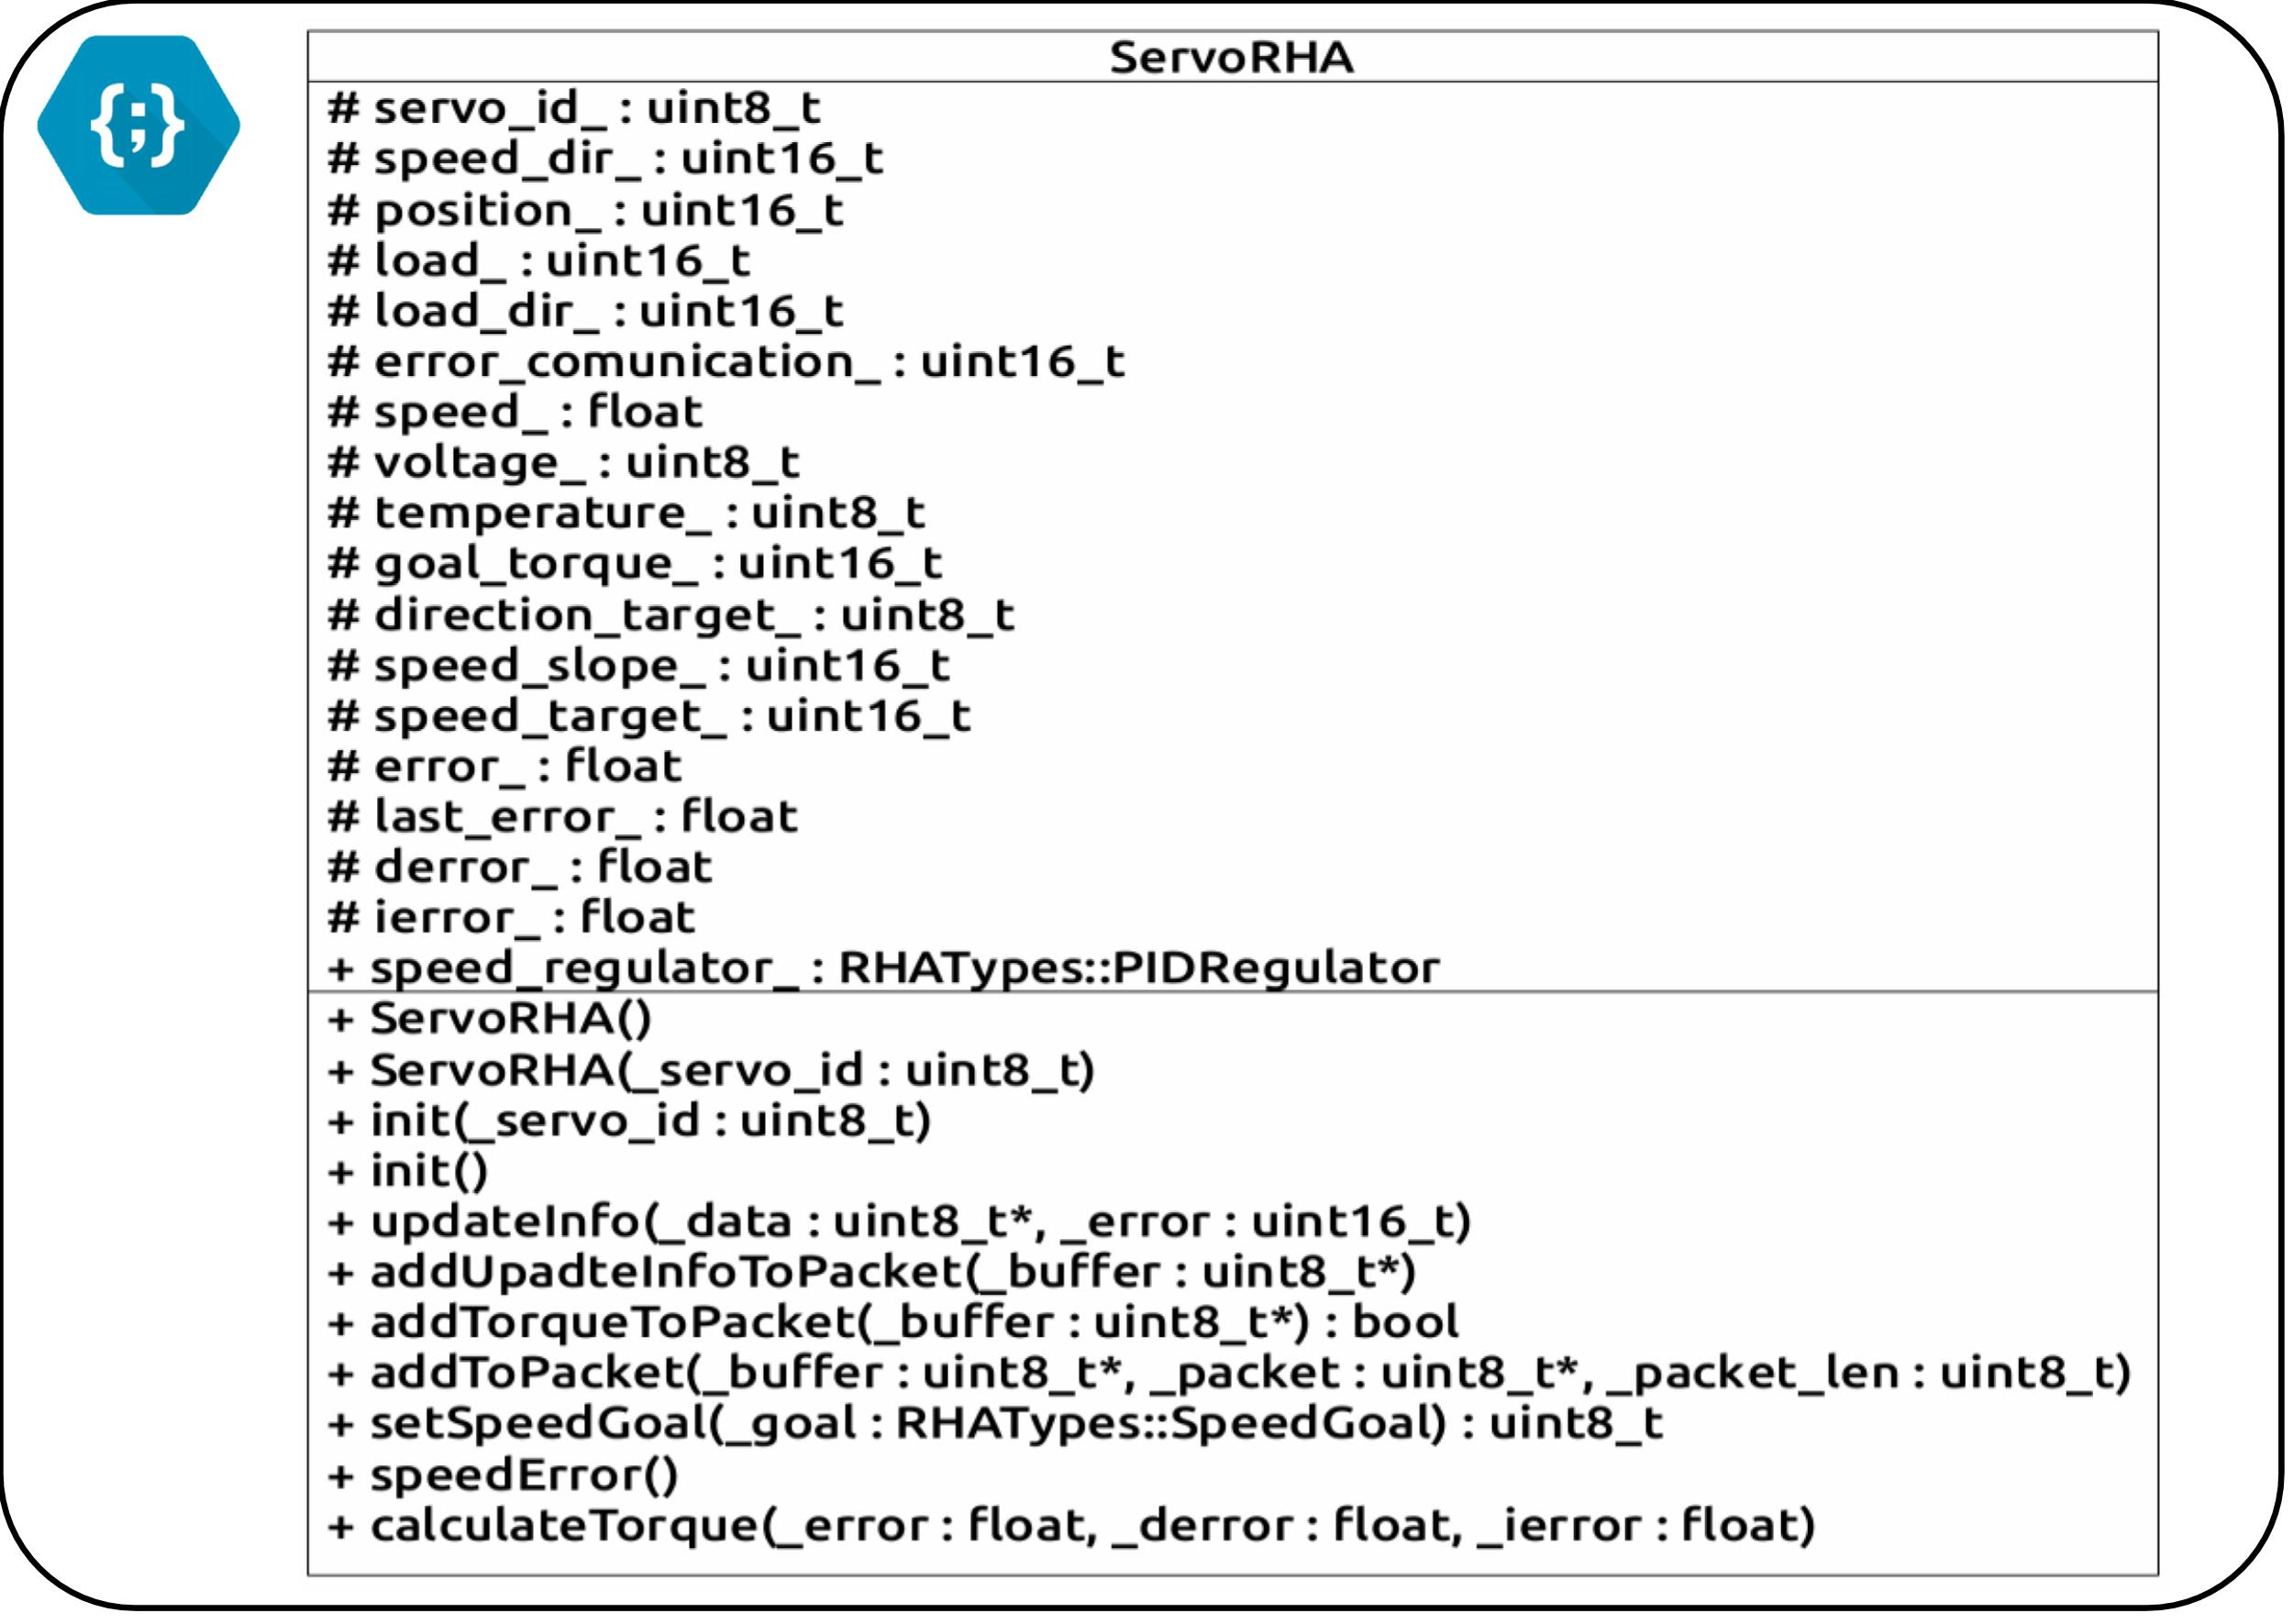
\includegraphics[width=0.8\textwidth]{figuras/Imagenes_SW/class_diagram_SRHA.jpg}
            \caption{Atributos y métodos más relevantes del objeto \textit{ServoRHA}}
            \label{fig:SW:class_diagram_SRHA}
            \immagesource{Autor}
        \end{figure}

        Se puede consultar información de más bajo nivel referente a este objeto así como a sus atributos y métodos en el Anexo \ref{app:documentacion_software} sección \completar.

    \subsection{Gestión de la información de la articulación} \label{subsec:SW:jointrha}
        Instanciando un objeto del tipo Servo el objeto tipo JointRHA (nombre dado en el proyecto) agrupa toda la información y funcionalidad referente a la articulación. De un modo análogo al caso descrito anteriormente implementa el control de posición efectuado sobre la articulación así como toda la matemática implicada.
        \\
        Este componetne recibe consignas de posición a alcanzar de forma que calcula la velocidad a requerir al servo, que será procesada por el objeto Servo descrito en \ref{subsec:SW:servorha}.
        \\
        En el diagrama de la figura \ref{fig:SW:class_diagram_SRHA} puede verse información genérica de la estructura implementada para este componente.
        \begin{figure}[H]
            \centering
            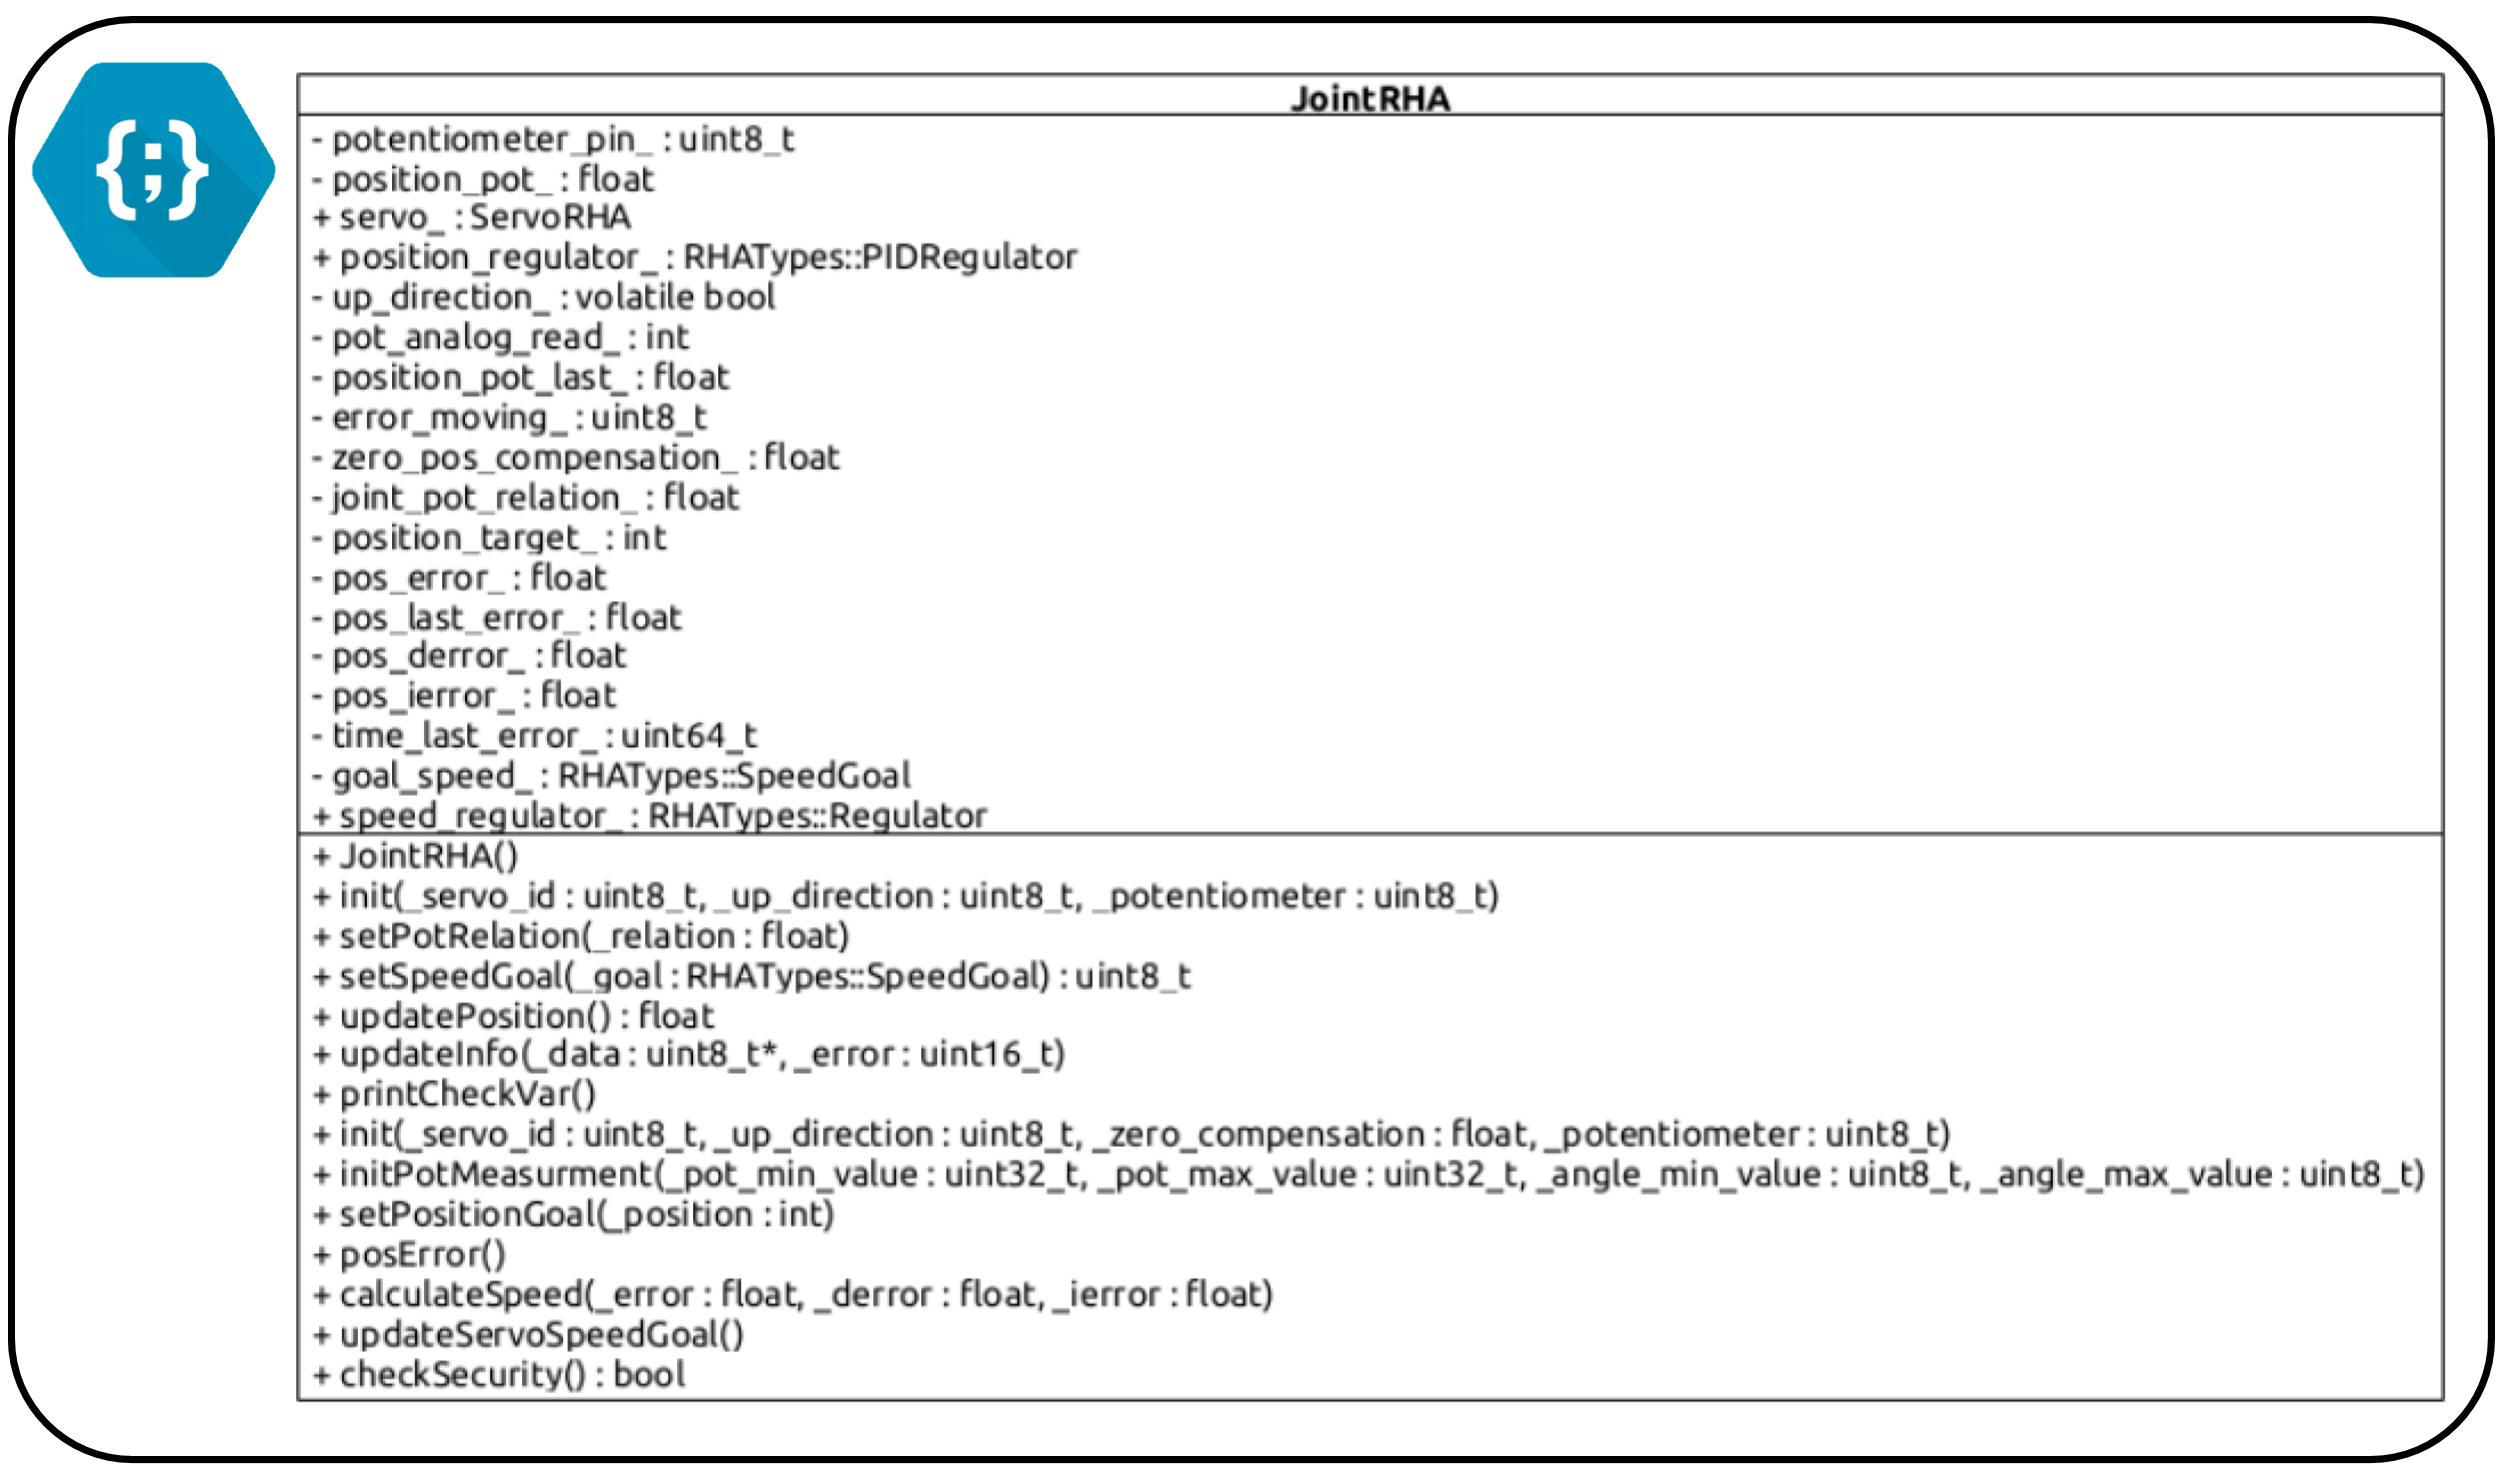
\includegraphics[width=0.100\textwidth]{figuras/Imagenes_SW/class_diagram_JRHA.jpg}
            \caption{Atributos y métodos más relevantes del objeto \textit{JointRHA}}
            \label{fig:SW:class_diagram_JRHA}
            \immagesource{Autor}
        \end{figure}

        Como en los casos anteriores se puede ampliar la información sobre este componente, a más bajo nivel, en el anexo \ref{app:documentacion_software} sección \completar.
    \subsection{Manejador de articulaciones} \label{subsec:SW:joint_handler}
        El componente encargado de gestionar y coordinar las funcionalidades descritas para los componentes ServoRHA y JointRHA es el conocido internamente como JointHandler. Este componente está a cargo de gestionar la comunicación con el puerto serie así como de gestionar los bucles de control de posición y velocidad.
        \\
        Para cumplir con su propósito instancia temporizadores como los descritos en el apartado \ref{subsec:SW:rhatypes} de forma que establece una frecuencia de funcionamiento concreta para cada lazo de control.
        \\
        Ambos lazos de control siguen una estructura similar cuyos pasos pueden resumirse en los siguientes, que solo se llevarán a cabo en caso de que no se haya detectado ningún error bloqueante.
        \begin{enumerate}
            \item Atualización de la información: todos los componentes de cada articulación actualizan su información suministrada por los servos físicos o por la realimentación correspondiente. En el caso del control de posición este paso se omite por asumir que, el lazo más veloz, ya ha actualizado la información.
            \item Realización de los cálculos correspondientes: el manejador va llamando a los componentes correspondientes para que, utilizando la información reunida en el paso anterio actualicen la consigna que se enviará.
            \item Asegurar la seguridad: un paso imprescindible en el cual se asegura que los datos que se van a enviar no ponen en riesgo la integridad del robot ni del paciente. Además se comprueba que los datos recibidos del entorno son coherentes, en caso contrario se almacena un marcador de error.
            \item Envio de comandos al siguiente nivel: una vez se cumplen los requisitos de seguridad se puede enviar la información al siguiente nivel. En el caso articular se pasa el objetivo de velocidad a los servos; en el caso de los objetos de tipo servo se envía la consigna de par obtenida a los servos físicos a través del puerto serie. En el caso concreto de exisir algún tipo de error se envía una señal de parada para todos los componentes inferiores.
        \end{enumerate}
        Se puede ver este comportamiento para el caso concreto del control de velocidad implementado para los servos en la figura \ref{fig:SW:joint_handler_loop}.

        \begin{figure}[H]
            \centering
            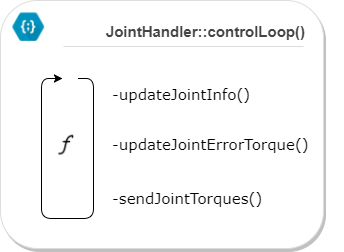
\includegraphics[width=0.45\textwidth]{figuras/Imagenes_SW/joint_handler_loop.png}
            \caption{Esquema de ejecución de bucle de control de joint\_handler}
            \label{fig:SW:joint_handler_loop}
            \immagesource{Autor}
        \end{figure}

        De igual forma se puede ver como se estructura el ciclo de control referente al control de posición articular en la figura \completar.

        El diagrama de clases de este componente, junto con los métodos y atributos más significativos se encuentran en la figura \ref{fig:SW:class_diagram_JH}.

        \begin{figure}[H]
            \centering
            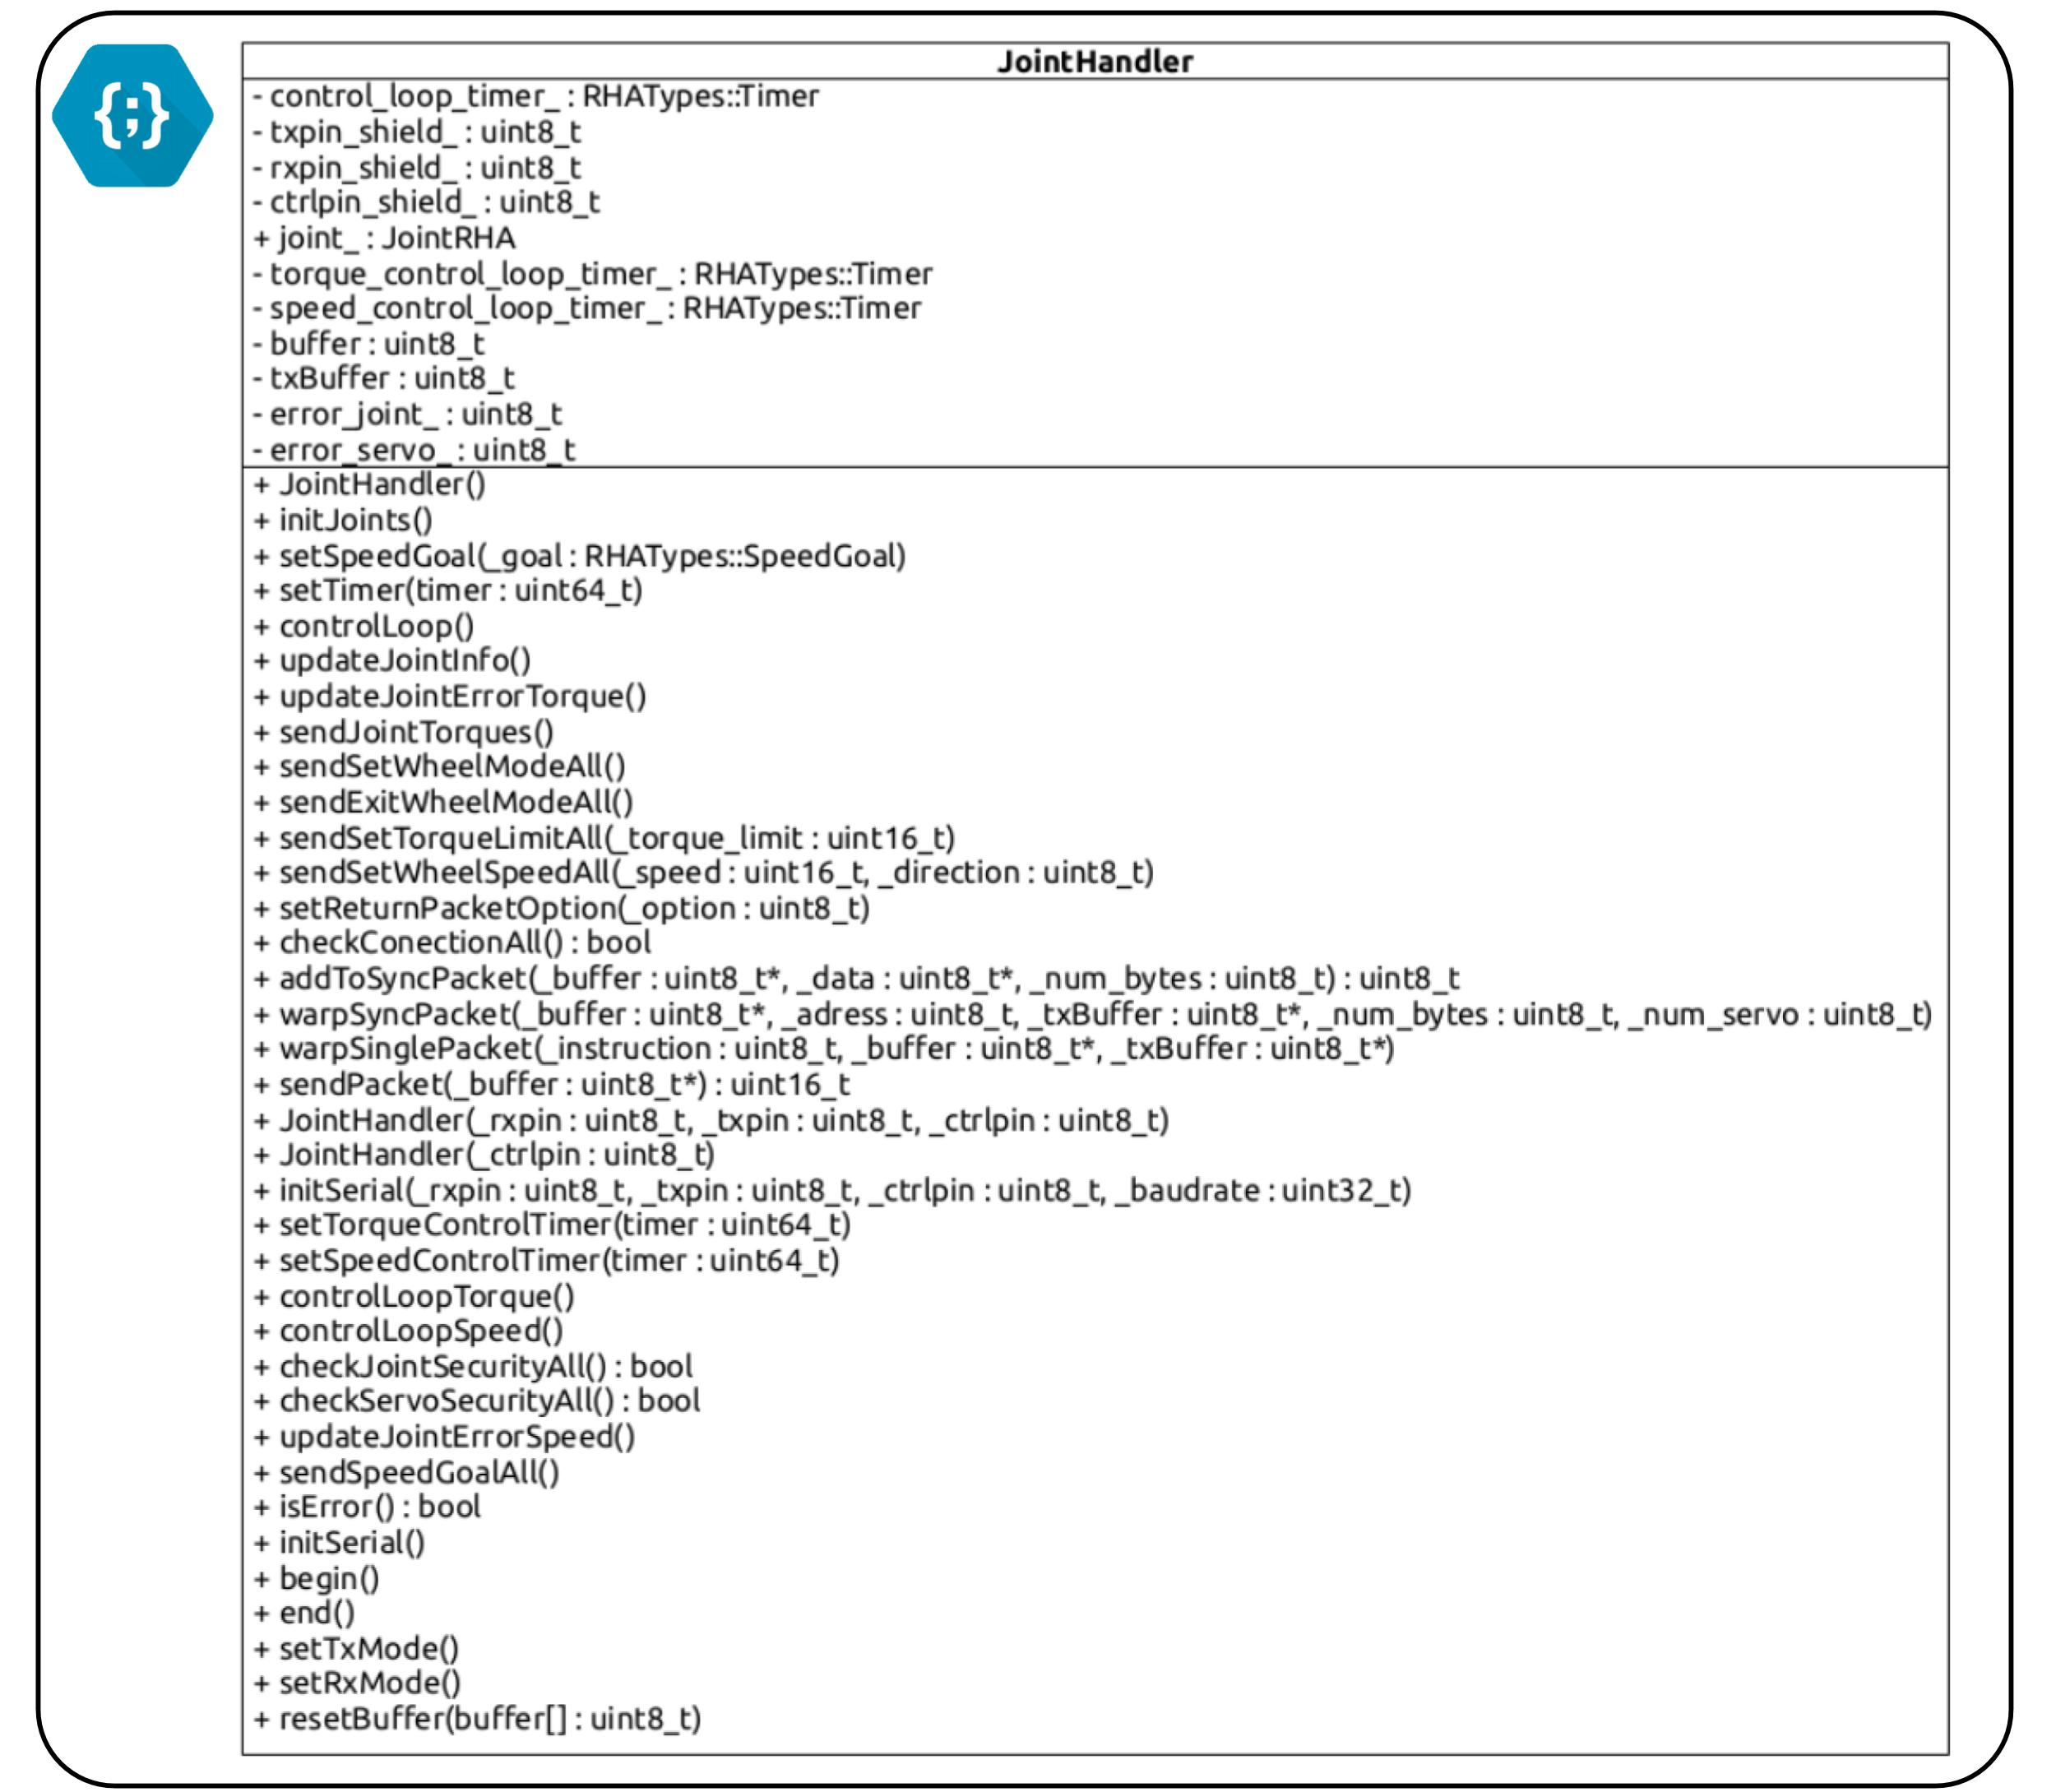
\includegraphics[width=1\textwidth]{figuras/Imagenes_SW/class_diagram_JH.jpg}
            \caption{Atributos y métodos más relevantes del objeto \textit{JointHandler}}
            \label{fig:SW:class_diagram_JH}
            \immagesource{Autor}
        \end{figure}

        Información más detallada sobre el componente puede encontrarse en el anexo \ref{app:documentacion_software} sección \completar.
    \subsection{Manejador del mando Nunchuck} \label{subsec:SW:chuck_handler}
        Se ha desarrollado un componente para permitir el control de los tres grados de libertad de posición, tal y como se han descrito en el capítulo \ref{chap:Mecanica}, a través de un mando Nunchuck de la consola Wii de Nintendo. Este componente no se ha incluido ni listado en la descripción de la electrónica por no ser un componente intrínseco al robot. El uso de este componente ha sido con fines puramente de test de las funcionalidades previa definición de una interfaz más estable.
        \\
        Este componente utiliza la librería \ingles{Wire} estandar de Arduino para comunicar con el mando y posteriormente traduce los valores recogidos en consignas de velocidad para las diferentes articulaciones a una frecuencia preestablecida. El diagrama correspndiente a este objeto se encuentra en la figura \ref{fig:SW:class_diagram_CHH}.

        \begin{figure}[H]
          	\centering
          	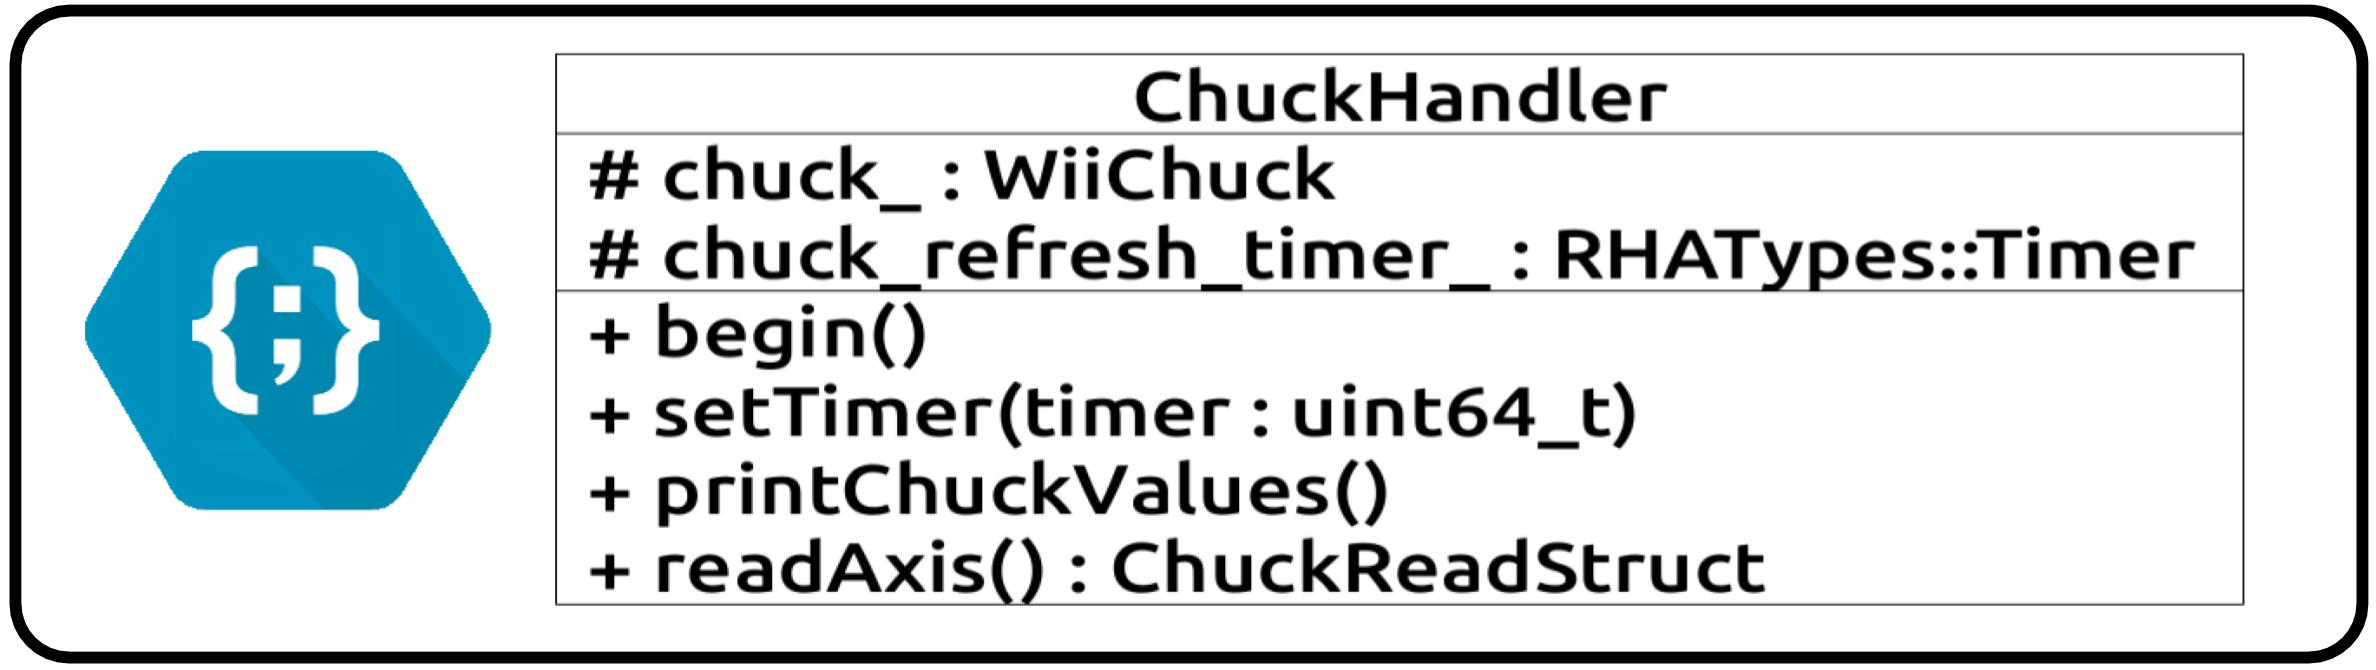
\includegraphics[width=0.65\textwidth]{figuras/Imagenes_SW/class_diagram_CHH.jpg}
          	\caption{Atributos y métodos más relevantes del objeto \textit{ChuckHandler}}
          	\label{fig:SW:class_diagram_CHH}
          	\immagesource{Autor}
        \end{figure}

    \subsection{Gestión del brazo robótico} \label{subsec:SW:robotrha}
        Este componente es el encargado de coordinar el resto de objetos descritos. Contiene la información de la cinemática vista en el capítulo \ref{chap:Cinematica} e implementa diferentes modos de funcionamiento o control del brazo robótico.
        \\
        El primer caso se ha adelantado en la descripción del manejador del Nunchuck de forma que se actualizan los comandos de velocidad de los servos a partir de la información obtenida del mando.
        \\
        Para una comunicación y control más complejo este componente implementa un protocolo de comunicación serie a través del cual se podrá establecer una comunicación con el brazo robótico desde componentes externos a través de un puerto serial estandar. En este caso se utiliza uno de los puertos series extra incluidos en la placa Arduino Mega, tal y como se ha descrito en el apartado \ref{sec:Electronica:Placa} dejando el puerto serie por defecto para funciones de carga del software así como \ingles{debug}.
        \\
        La interfaz principal de este componente se puede ver en el diagrama de la figura \completar pudiendo ampliar la información del mismo en el anexo \ref{app:documentacion_software} sección \completar.
        \\
        El protocolo de comunicación implementado para interactuar con el brazo robótico está descrito en el anexo \completar
    \subsection{Fichero fuente principal} \label{subsec:SW:maincpp}

\section{Test y verificación del software} \label{sec:SW:test}

\section{Gestión de la complejidad y mantenibilidad} \label{sec:SW:gestion_complejidad}

    \subsection{Comprobación del cumplimiento de las reglas de codificación del Código}
